%Copyright (c) 2017 Davide Quattrocchi All Rights Reserved.
\documentclass[a4paper,10pt]{report} % Prepara un documento per carta A4, con un bel font grande
\usepackage[italian]{babel} % Adatta LaTeX alle convenzioni tipografiche italiane,
% e ridefinisce alcuni titoli in italiano, come "Capitolo" al posto di "Chapter",
%\usepackage[T1]{fontenc} % Riga da togliere se si compila con PDFLaTeX
\usepackage[utf8]{inputenc} % Consente l'uso caratteri accentati italiani
\usepackage{graphicx, floatflt, eso-pic}
\frenchspacing% forza LaTeX ad una spaziatura uniforme, invece di lasciare più spazio
              % alla fine dei punti fermi come da convenzione inglese
\makeatletter\patchcmd{\l@chapter}{1.0em}{0.3em}{}{}\makeatother %riduco la spaziatura
% dei capitoli da 1.0 a 0.3 per fare entrare l'indice tutto in una pagina
\makeatletter\@addtoreset{chapter}{part}\makeatother% modifico la numerazione dei capitoli
                                                    % per resettarla all'interno di ogni parte
\begin{document}
\begin{titlepage}% pagina I
	\centering
	%\vspace{1.5cm}
	\vfill
	%{\AddToShipoutPicture*{\AtPageCenter{\makebox(0 ,0)
	%	{\includegraphics[width=0.9\paperwidth,height=0.9\paperheight,keepaspectratio=false]{logoUniUrb}}}}}
	%\includegraphics[height=8mm]{Kode-simbol.jpg}
	{\huge\bfseries N2L - Need 2 Log\par}
  \vspace{1cm}
  {\scshape\large\itshape Programma di utility per lo storage di credenziali personali.\par}
	\vspace{0.5cm}
  {\scshape\large Relazione del progetto di P.O.I.S.\par}
	\vspace{2cm}
	{\Large\itshape Davide Quattrocchi\par}
  {\large MATRICOLA: 273654\par}
	{\itshape d.quattrocchi@campus.uniurb.it\par}
	\vfill
  {\large A.A.:2016/17\par}
	\vspace{0.2cm}
	Professore: ~Edoardo \textsc{Bontà}\par
	\vspace{1.0cm}
	~Università degli Studi di Urbino \textsc{"Carlo Bo"}\par
	\vfill
  %Bottom of the page
  \vspace{0.5cm}
  Questo documento è stato preparato con \LaTeX.
  \end{titlepage}
\newpage
\tableofcontents % Prepara l'indice generale - pagina 1
\newpage
\chapter{Specifica del problema} %Prima parte - pagina
		Si vuole realizzare un sistema che dia la possibilità di salvare in modo sicuro
			gli account posseduti dall'utilizzatore in modo tale che egli non debba ricordare
			ogni singola credenziale, username o password personale.

		Per poter rispettare suddetta specifica, il sistema dovrà possedere tali
		 	caratteristiche e comportamenti:
		\begin{itemize}
			\item Tutti i dati sensibili forniti dall'utente dovranno essere salvati
				all'interno di un database criptato.
			\item L'accesso al sistema deve essere permesso solo dopo l'immissione e la
				verifica di una passphrase.
			\item La password di accesso deve essere conservata in modo sicuro.
			\item L'accesso all'applicativo e ai dati potrà essere eseguito solo dopo che
				l'utilizzatore avrà inserito la corretta passphrase (da lui preventivamente
				definita).
			\item Il sistema deve dare la possibilità di modificare ed eliminare uno o
				tutti i dati presenti nel database.
			\item Il sistema deve permettere di cambiare le impostazioni dell'applicazione,
				tra cui anche la password di accesso.
			\end{itemize}
\newpage
\chapter{Specifica dei requisiti} %
	Osservando la specifica del problema risulta evidente quanto l’applicazione
	debba possedere efficienti sistemi di sicurezza, per preservare i dati dell’utilizzatore
	da un eventuale attacco informatico.\vfill
	In particolare, si è deciso di proteggere le informazioni che l’utente affida
	al sistema utilizzando questi metodi:\vfill
	\begin{itemize}
			\item La passphrase di accesso al programma non verrà conservata in chiaro
				tra le impostazioni della applicazione, ma ne verrà conservato solamente l’hash,
				calcolato tramite l’algoritmo SHA-256.
			\item La password in questione verrà utilizzata come chiave di de/criptazione del database:
				così facendo, se anche un malintenzionato riuscisse a superare la prima fase di controllo
				alterando l’hash o tramite una collisione, non gli sarebbe possibile ottenere i dati corretti
				poiché questi verrebbero decriptati con una chiave errata.
			\item	L’applicazione può permettere di cambiare la password di accesso al sistema da parte dell’utente,
				così che l’utilizzatore riduca le probabilità che un attaccante riesca a sorpassare i
				sistemi di sicurezza tramite attacchi basati su associazioni e confronti
				(bruteforcing, dictionary attack, rainbow tables attack, ecc).
			\item	In fase di modifica della password, l’utente può decidere di inserire una
			propria password personale o di crearne una pseudo randomicamente tramite un
			apposito algoritmo messo a disposizione dal sistema stesso.
		\end{itemize}
  \section{cap 1}
    Lorem ipsum dolor sit amet, consectetur adipisicing elit, sed do eiusmod tempor incididunt ut labore et dolore magna aliqua. Ut enim ad minim veniam, quis nostrud exercitation ullamco laboris nisi ut aliquip ex ea commodo consequat. Duis aute irure dolor in reprehenderit in voluptate velit esse cillum dolore eu fugiat nulla pariatur. Excepteur sint occaecat cupidatat non proident, sunt in culpa qui officia deserunt mollit anim id est laborum.
  \section{Diagramma dei casi d'uso}
    Si riportano di seguito i casi d'uso relativi alla libreria (...) e all'interfaccia grafica.
		\begin{figure}[htbp]
			\centering
			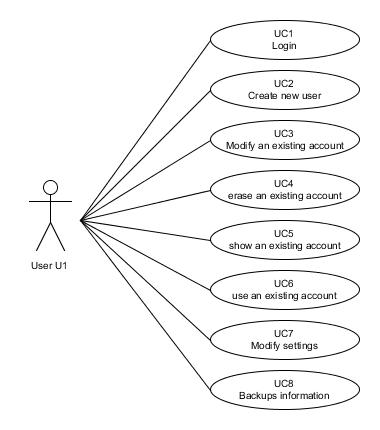
\includegraphics[scale = 0.5]{immagini/USE_CASE_DIAGRAM-UMLet.jpg}
			\caption{Diagramma dei casi d'uso tramite GUI da parte dell'utente}
			\end{figure}
  \section{Template dei casi d'uso}
		Nel capitolo 5 si descriverà un test black-box relativo all’interfaccia dimostrativa,
			vengono pertanto riportati qui tutti i template dei casi d’uso relativi.

		Poiché il processo di sviluppo utilizzato (sezione 4.1) prevede lo sviluppo orientato ai test,
			non è necessario effettuare dei test di tipo black-box sulla libreria
			(durante lo sviluppo vengono creati test white-box che coprono quasi tutti i possibili flussi d’esecuzione)
			ed è quindi superfluo descrivere i template dei casi d’uso della libreria.

		\begin{figure}[htbp]
			\centering
			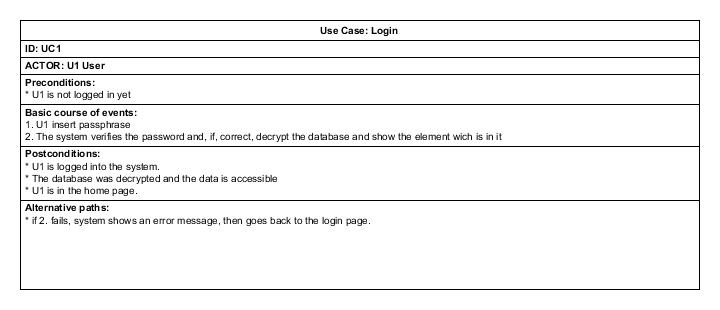
\includegraphics[width = \textwidth]{immagini/USE_CASE_TEMPLATE/UC01.jpg}
			\caption{Template relativo al caso d'uso UC1}
			\end{figure}
		\begin{figure}[htbp]
			\centering
			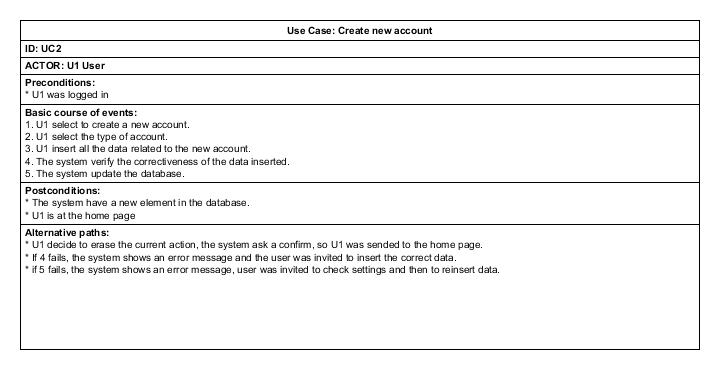
\includegraphics[width = \textwidth]{immagini/USE_CASE_TEMPLATE/UC02.jpg}
			\caption{Template relativo al caso d'uso UC2}
			\end{figure}
		\begin{figure}[htbp]
			\centering
			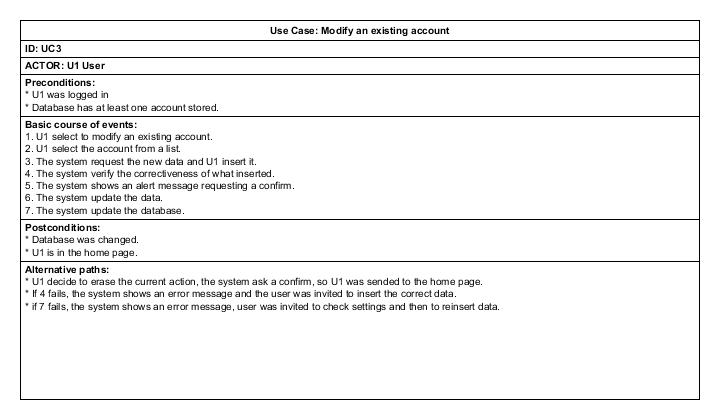
\includegraphics[width = \textwidth]{immagini/USE_CASE_TEMPLATE/UC03.jpg}
			\caption{Template relativo al caso d'uso UC3}
			\end{figure}
		\begin{figure}[htbp]
			\centering
			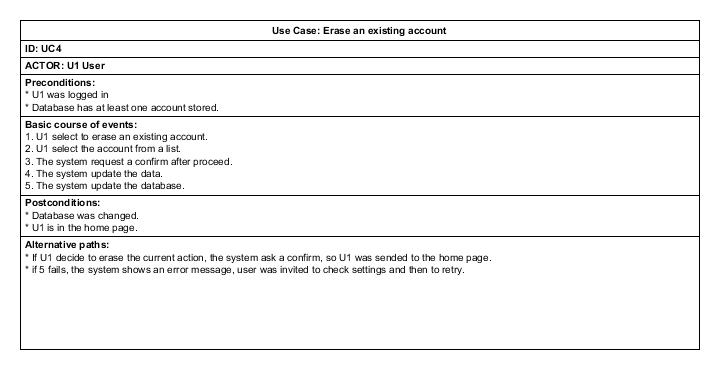
\includegraphics[width = \textwidth]{immagini/USE_CASE_TEMPLATE/UC04.jpg}
			\caption{Template relativo al caso d'uso UC4}
			\end{figure}
		\begin{figure}[htbp]
			\centering
			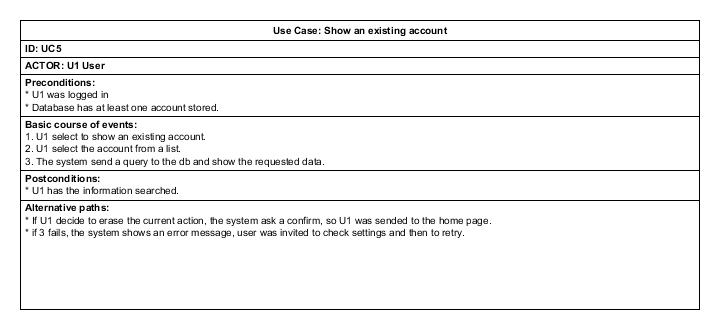
\includegraphics[width = \textwidth]{immagini/USE_CASE_TEMPLATE/UC05.jpg}
			\caption{Template relativo al caso d'uso UC5}
			\end{figure}
		\begin{figure}[htbp]
			\centering
			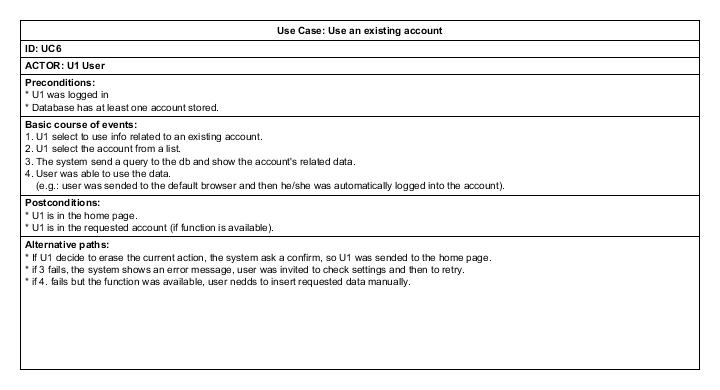
\includegraphics[width = \textwidth]{immagini/USE_CASE_TEMPLATE/UC06.jpg}
			\caption{Template relativo al caso d'uso UC6}
			\end{figure}
		\begin{figure}[htbp]
			\centering
			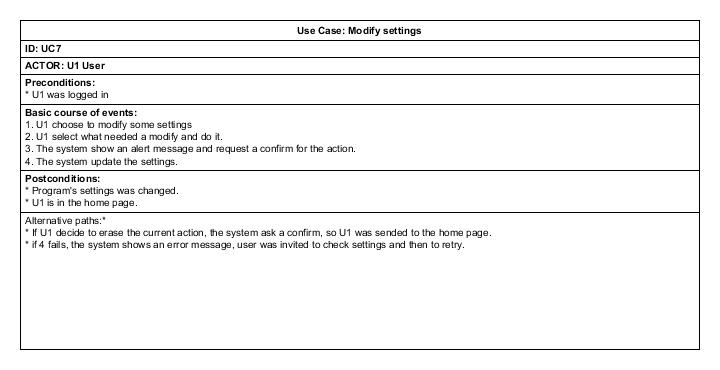
\includegraphics[width = \textwidth]{immagini/USE_CASE_TEMPLATE/UC07.jpg}
			\caption{Template relativo al caso d'uso UC7}
			\end{figure}
		\begin{figure}[htbp]
			\centering
			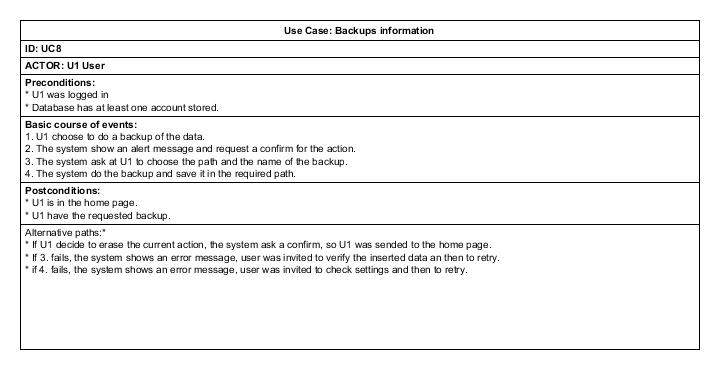
\includegraphics[width = \textwidth]{immagini/USE_CASE_TEMPLATE/UC08.jpg}
			\caption{Template relativo al caso d'uso UC8}
			\end{figure}
  \section{cap 4}
    Lorem ipsum dolor sit amet, consectetur adipisicing elit, sed do eiusmod tempor incididunt ut labore et dolore magna aliqua. Ut enim ad minim veniam, quis nostrud exercitation ullamco laboris nisi ut aliquip ex ea commodo consequat. Duis aute irure dolor in reprehenderit in voluptate velit esse cillum dolore eu fugiat nulla pariatur. Excepteur sint occaecat cupidatat non proident, sunt in culpa qui officia deserunt mollit anim id est laborum.
\newpage
\chapter{Analisi e progettazione} %
	Per la realizzazione dei requisiti verrà utilizzato il linguaggio di programmazione C#.
	
  \section{GUI}
			Per la realizzazione della interfaccia grafica della applicazione, si è deciso
			di utilizzare le librerie Microsoft Windows Forms, del framework Microsoft .NET
  \section{cap 2}
    Lorem ipsum dolor sit amet, consectetur adipisicing elit, sed do eiusmod tempor incididunt ut labore et dolore magna aliqua. Ut enim ad minim veniam, quis nostrud exercitation ullamco laboris nisi ut aliquip ex ea commodo consequat. Duis aute irure dolor in reprehenderit in voluptate velit esse cillum dolore eu fugiat nulla pariatur. Excepteur sint occaecat cupidatat non proident, sunt in culpa qui officia deserunt mollit anim id est laborum.
  \section{cap 3}
    Lorem ipsum dolor sit amet, consectetur adipisicing elit, sed do eiusmod tempor incididunt ut labore et dolore magna aliqua. Ut enim ad minim veniam, quis nostrud exercitation ullamco laboris nisi ut aliquip ex ea commodo consequat. Duis aute irure dolor in reprehenderit in voluptate velit esse cillum dolore eu fugiat nulla pariatur. Excepteur sint occaecat cupidatat non proident, sunt in culpa qui officia deserunt mollit anim id est laborum.
  \section{cap 4}
    Lorem ipsum dolor sit amet, consectetur adipisicing elit, sed do eiusmod tempor incididunt ut labore et dolore magna aliqua. Ut enim ad minim veniam, quis nostrud exercitation ullamco laboris nisi ut aliquip ex ea commodo consequat. Duis aute irure dolor in reprehenderit in voluptate velit esse cillum dolore eu fugiat nulla pariatur. Excepteur sint occaecat cupidatat non proident, sunt in culpa qui officia deserunt mollit anim id est laborum.
\newpage
\chapter{Implementazione} %
  La forza di \LaTeX\ sono però le formule, sia in linea (ad esempio \(y=x^2\))
   che messe in bella mostra in un'area propria:
  \[y=\sqrt{x+y}\]
  \section{cap 1}
    Lorem ipsum dolor sit amet, consectetur adipisicing elit, sed do eiusmod tempor incididunt ut labore et dolore magna aliqua. Ut enim ad minim veniam, quis nostrud exercitation ullamco laboris nisi ut aliquip ex ea commodo consequat. Duis aute irure dolor in reprehenderit in voluptate velit esse cillum dolore eu fugiat nulla pariatur. Excepteur sint occaecat cupidatat non proident, sunt in culpa qui officia deserunt mollit anim id est laborum.
  \section{cap 2}
    Lorem ipsum dolor sit amet, consectetur adipisicing elit, sed do eiusmod tempor incididunt ut labore et dolore magna aliqua. Ut enim ad minim veniam, quis nostrud exercitation ullamco laboris nisi ut aliquip ex ea commodo consequat. Duis aute irure dolor in reprehenderit in voluptate velit esse cillum dolore eu fugiat nulla pariatur. Excepteur sint occaecat cupidatat non proident, sunt in culpa qui officia deserunt mollit anim id est laborum.
  \section{cap 3}
    Lorem ipsum dolor sit amet, consectetur adipisicing elit, sed do eiusmod tempor incididunt ut labore et dolore magna aliqua. Ut enim ad minim veniam, quis nostrud exercitation ullamco laboris nisi ut aliquip ex ea commodo consequat. Duis aute irure dolor in reprehenderit in voluptate velit esse cillum dolore eu fugiat nulla pariatur. Excepteur sint occaecat cupidatat non proident, sunt in culpa qui officia deserunt mollit anim id est laborum.
\newpage
\chapter{Test} %
  La forza di \LaTeX\ sono però le formule, sia in linea (ad esempio \(y=x^2\))
   che messe in bella mostra in un'area propria:
  \[y=\sqrt{x+y}\]
  \section{cap 1}
    Lorem ipsum dolor sit amet, consectetur adipisicing elit, sed do eiusmod tempor incididunt ut labore et dolore magna aliqua. Ut enim ad minim veniam, quis nostrud exercitation ullamco laboris nisi ut aliquip ex ea commodo consequat. Duis aute irure dolor in reprehenderit in voluptate velit esse cillum dolore eu fugiat nulla pariatur. Excepteur sint occaecat cupidatat non proident, sunt in culpa qui officia deserunt mollit anim id est laborum.
    \subsection{sez 1}
      Lorem ipsum dolor sit amet, consectetur adipisicing elit, sed do eiusmod tempor incididunt ut labore et dolore magna aliqua. Ut enim ad minim veniam, quis nostrud exercitation ullamco laboris nisi ut aliquip ex ea commodo consequat. Duis aute irure dolor in reprehenderit in voluptate velit esse cillum dolore eu fugiat nulla pariatur. Excepteur sint occaecat cupidatat non proident, sunt in culpa qui officia deserunt mollit anim id est laborum.
  \section{cap 2}
    Lorem ipsum dolor sit amet, consectetur adipisicing elit, sed do eiusmod tempor incididunt ut labore et dolore magna aliqua. Ut enim ad minim veniam, quis nostrud exercitation ullamco laboris nisi ut aliquip ex ea commodo consequat. Duis aute irure dolor in reprehenderit in voluptate velit esse cillum dolore eu fugiat nulla pariatur. Excepteur sint occaecat cupidatat non proident, sunt in culpa qui officia deserunt mollit anim id est laborum.
    \subsection{sez 2}
      Lorem ipsum dolor sit amet, consectetur adipisicing elit, sed do eiusmod tempor incididunt ut labore et dolore magna aliqua. Ut enim ad minim veniam, quis nostrud exercitation ullamco laboris nisi ut aliquip ex ea commodo consequat. Duis aute irure dolor in reprehenderit in voluptate velit esse cillum dolore eu fugiat nulla pariatur. Excepteur sint occaecat cupidatat non proident, sunt in culpa qui officia deserunt mollit anim id est laborum.
\newpage
\chapter{Compilazione ed esecuzione} %
	La forza di \LaTeX\ sono però le formule, sia in linea (ad esempio \(y=x^2\))
   che messe in bella mostra in un'area propria:
  \[y=\sqrt{x+y}\]
  \section{cap 1}
    Lorem ipsum dolor sit amet, consectetur adipisicing elit, sed do eiusmod tempor incididunt ut labore et dolore magna aliqua. Ut enim ad minim veniam, quis nostrud exercitation ullamco laboris nisi ut aliquip ex ea commodo consequat. Duis aute irure dolor in reprehenderit in voluptate velit esse cillum dolore eu fugiat nulla pariatur. Excepteur sint occaecat cupidatat non proident, sunt in culpa qui officia deserunt mollit anim id est laborum.
    \subsection{sez 1}
      Lorem ipsum dolor sit amet, consectetur adipisicing elit, sed do eiusmod tempor incididunt ut labore et dolore magna aliqua. Ut enim ad minim veniam, quis nostrud exercitation ullamco laboris nisi ut aliquip ex ea commodo consequat. Duis aute irure dolor in reprehenderit in voluptate velit esse cillum dolore eu fugiat nulla pariatur. Excepteur sint occaecat cupidatat non proident, sunt in culpa qui officia deserunt mollit anim id est laborum.
  \section{cap 2}
    Lorem ipsum dolor sit amet, consectetur adipisicing elit, sed do eiusmod tempor incididunt ut labore et dolore magna aliqua. Ut enim ad minim veniam, quis nostrud exercitation ullamco laboris nisi ut aliquip ex ea commodo consequat. Duis aute irure dolor in reprehenderit in voluptate velit esse cillum dolore eu fugiat nulla pariatur. Excepteur sint occaecat cupidatat non proident, sunt in culpa qui officia deserunt mollit anim id est laborum.
    \subsection{sez 1}
      Lorem ipsum dolor sit amet, consectetur adipisicing elit, sed do eiusmod tempor incididunt ut labore et dolore magna aliqua. Ut enim ad minim veniam, quis nostrud exercitation ullamco laboris nisi ut aliquip ex ea commodo consequat. Duis aute irure dolor in reprehenderit in voluptate velit esse cillum dolore eu fugiat nulla pariatur. Excepteur sint occaecat cupidatat non proident, sunt in culpa qui officia deserunt mollit anim id est laborum.
\end{document}
